\documentclass[12pt,a4paper]{article}
\usepackage[utf8]{inputenc}
\usepackage[russian]{babel}
\usepackage[OT1]{fontenc}
\usepackage{mathtools}
\usepackage{amsfonts}
\usepackage{amssymb}
\usepackage{enumitem}
\usepackage{alltt}
\usepackage{graphicx}
\usepackage{indentfirst}
\usepackage{caption}
\usepackage{float}
\usepackage{wrapfig}
\setlength{\parindent}{0.75cm}
\graphicspath{{pictures/}}
\DeclareGraphicsExtensions{.png}
\usepackage[left=15mm,right=15mm,top=2cm,bottom=2cm]{geometry}
\author{Глотов Алексей}
\begin{document}
\newpage
\begin{center}
\footnotesize{{ГОСУДАРСТВЕННОЕ АВТОНОМНОЕ ОБРАЗОВАТЕЛЬНОЕ УЧРЕЖДЕНИЕ}\break
{ВЫСШЕГО ОБРАЗОВАНИЯ}
\break
{\bf {МОСКОВСКИЙ ФИЗИКО-ТЕХНИЧЕСКИЙ ИНСТИТУТ}}
\break
\small{(НАЦИОНАЛЬНЫЙ ИССЛЕДОВАТЕЛЬСКИЙ УНИВЕРСИТЕТ)}}
\break
\hfill \break
\hfill \break
\begin{center}
\normalsize{Кафедра общей физики}
\end{center}
\hfill \break
\hfill \break
\hfill \break
\hfill \break

\begin{center}
\normalsize {Лабораторная работа 1.2.5}
\end{center}
\hfill \break\\
\large{Исследование прецессии уравновешенного гироскопа}
\end{center}
\begin{flushleft}
\hfill \break
\hfill \break
\hfill \break
\hfill \break
\hfill \break
\hfill \break
\hfill \break
\hfill \break
\hfill \break
\hfill \break
\hangindent=9cm
\normalsize{Преподаватель:}\hfill
\normalsize{к.ф.-м.н., доц. Яворский В.А.}\\
\hfill \break
\normalsize{Обучающийся:}\hfill
\normalsize{Глотов А.А.} \\
\hfill \break
\end{flushleft}
\hfill \break
\hfill \break
\hfill \break
\hfill \break
\hfill \break
\hfill \break
\hfill \break
\hfill \break
\hfill \break
\hfill \break
\hfill \break

\begin{center}
Долгопрудный \break
 2021
\end{center}
\thispagestyle{empty}
\newpage
\begin{center}
\large{\bf Введение} 
\end{center}
\begin{center}
\large{Цели работы} \break
\end{center}
\begin{itemize}
\item Исследовать вынужденную прецессию гироскопа
\item Установить зависимость скорости вынужденной прецессии гироскопа от величины момента сил, действующих на ось гироскопа
\item Определить сокрость вращения ротора гироскопа и сравнить ее со скоростью, рассчитанной по скорости прецессии 
\end{itemize}
\hfill \break
\begin{center}
\large{Приборы и материалы}
\end{center}
\begin{enumerate}
\item Гироскоп в кардановом подвесе
\item Секундомер	
\item Набор грузов
\item Отдельный ротор гироскопа
\item Цилиндр известной массы (Цилиндр + весы)
\item Крутильный маятник
\item Штангенциркуль 
\item Линейка
\end{enumerate}
\newpage
\begin{center}
\large{Теоретические сведения}
\end{center}
\hfill
\begin{par}
Уравнения движения твёрдого тела можно записать в виде
\end{par}
\begin{equation}
\frac{d\vec{p}}{dt}=\vec{F} \label{1}
\end{equation}
\begin{equation}
\frac{d\vec{L}}{dt}=\vec{M} \label{2}
\end{equation}
\begin{par}
Уравнений \ref{1} и \ref{2} достаточно для описания движения твердого тела
\end{par}
\par Момент импульса твердого тела по главным осям x, y, z равен
\begin{equation}
\vec{L}=\vec{i}I_{x}\omega_{x}+\vec{j}I_{y}\omega_{y}+\vec{k}I_{z}\omega_{z} \label{3}
\end{equation}
где $I_{x}, I_{y}, I_{z}$ - главные моменты инерции, $\omega_{x}, \omega_{y}, \omega_{z}$ - компоненты вектора угловой скорости. Для гироскопа справедливо, что 
\begin{center}
$I_{z}\omega_{z} \gg I_{x}\omega_{x}, I_{y}\omega_{y}$ 
\end{center}
\par В силу \ref{2}, приращение момента импульса определяется интегралом
\begin{equation}
\Delta\vec{L}=\int \vec{M}dt \label{4}
\end{equation}
\par Если момент внешних сил действует в течение короткого промежутка времени, то
\begin{center}
$|\Delta\vec{L}| \ll |\vec{L}|$
\end{center}
С этим связана устойчивость быстро вращающегося гироскопа. В случае, если центр масс неподвижен, гироскоп называют уравновешенным 
\begin{figure}[H]
\centering
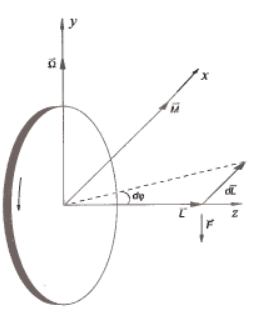
\includegraphics[width=9cm, height=9cm]{1.2.5_1}
\caption{Маховик}
\label{рис.1}
\end{figure}
\begin{par}
Рассмотрим маховик, изображенный на рис.\ref{рис.1}, вращающийся вокруг оси Oz, перпендикулярной к плоскости маховика. Будем считать, что 
\end{par}
\begin{center}
$\omega_{z}=\omega_{0}, \;\;\;\; \omega_{x}=\omega_{y}=0 $
\end{center}
Пусть ось повернулась в плоскости xOz по направлению к Ox на бесконечно малый угол $d\phi$. Такой поворот означает добавочное вращение маховика вокруг оси Oy, так что 
\begin{center}
$d\phi=\Omega{dt}$
\end{center}
где $\Omega$ - угловая скорость такого вращения. Будем предполагать, что 
\begin{equation}
L_{\Omega} \ll L_{\omega_{0}} \label{5}
\end{equation}
Это означает, что момент импульса маховика, равный $I_{z}\omega_{z}$ до приложения внешних сил, только повернутся в плоскости xOz по направлению к оси Ox не изменяя своей величины. Таким образом,
\begin{center}
$|d\vec{L}|=Ld\phi=L\Omega{dt}$
\end{center}
Изменение направлено вдоль Ox, поэтому 
\begin{center}
$d\vec{L}=[\vec{\Omega},\vec{L}]dt$
\end{center}
В силу \ref{2} имеем:
\begin{equation}
\vec{M}=[\vec{\Omega}, \vec{L}] \label{6}
\end{equation}
\par Для гироскопа массой $m_{г}$, у которого ось собственного вращения наклонена на угол $\alpha$ от вертикали, скорость прецессии равна
\begin{equation}
\Omega=\frac{M}{I_{z}\omega_{z}\sin{\alpha}}=\frac{m_{г}gl_{ц}\sin{\alpha}}{I_{z}\omega_{0}\sin{\alpha}}=\frac{m_{г}gl_{ц}}{I_{z}\omega_{0}} \label{7}
\end{equation}
$l_{ц}$ - расстояние от точки подвеса до центра масс гироскопа
\par Для изучения регулярной прецессии гироскопа используют к его оси подвешивают дополительные грузы. Тогда скорость прецессии
\begin{equation}
\Omega=\frac{mgl}{I_{z}\omega_{0}} \label{8}
\end{equation}
m - масса груза, l - расстояние от центра карданова подвеса до точки крепления груза на оси гироскопа рис.\ref{рис.2}
\begin{figure}[H]
\centering
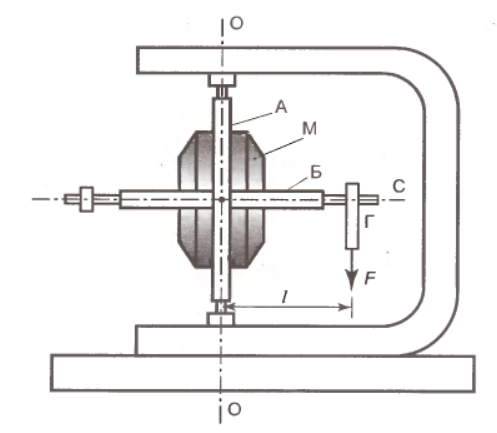
\includegraphics[width=12cm, height=9cm]{1.2.5_2}
\caption{Схема экспериментальной установки}
\label{рис.2}
\end{figure}
\begin{figure}[H]
\centering
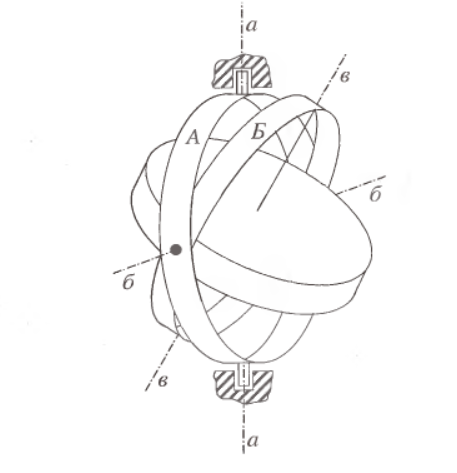
\includegraphics[width=12cm, height=9cm]{1.2.5_3}
\caption{Гироскоп в кардановом подвесе}
\label{рис.3}
\end{figure}
\par Измерение скорости прецессии гироскопа позволяет вычислить угловую скорость вращения его ротора (с помощью формулы \ref{8}). Момент инерции ротора относительно оси симметрии $I_{0}$ измеряется по крутильным колебаниям копии ротора, подвешенной вдоль оси симметрии на проволоке. Период считается по формуле 
\begin{equation}
T_{0}=2\pi\sqrt{\frac{I_{0}}{f}} \label{8}
\end{equation}
\par Для исключения неизвестной величины - модуля кручения проволоки, - к той же проволоке подвешивают цилиндр с известными массой и диаметром сечения, для которого легко считается момент инерции $I_{\text{ц}}$. Тогда момент инерции ротора $I_{0}$ определяется по формуле
\begin{equation}
I_{0}=I_{\text{ц}}\frac{T^2_{0}}{T^2_{ц}}
\end{equation} 
\newpage
\begin{center}
\large Ход работы
\end{center}
1) \par \large Рассмотрим реакцию гироскопа на воздействие внешних сил. Согласно теории, описывающей поведение гироскопа, направление отклонения должно совпадать с направдлением действия момента прикладываемой силы. Прикладывая силы перпендикулярно рычагу (очевидно, что в таком случае они также будут перпендикулярны плечу силы), отметим, что гироскоп действительно отколняется перпендикулярно рычагу и направлению действия силы. Несложно подтвердить, что направление отклонения совпадает с направлением вектора $[\vec{r},\vec{F}]$, т.е. удовлетворяет теоретическим данным \hfill \break
2)\par Подвесим к рычагу груз. Отметим начавшуюся  прецессию гироскопа, а также медленное горизонтальное (вниз) движение гироскопа из-за трения в оси карданвого подвеса (aa на рис.\ref{рис.3}) \hfill \break
3) \par Измерим скорость прецессии гироскопа в зависимости от массы груза, подвешенного на рычаг, параллельно замеряя скорость опускания рычага гироскопа. \break
\par Будем считать период прецессии гироскопа как время, необходимое для опускания на 10-12 градусов, за которое он совершит целое число оборотов, деленное на число оборотов \hfill \break
l = 12,2 см \;\;\;\;\; $\Delta{l}=0.1$см \hfill \break
\begin{center}
\begin{large}
\begin{tabular}{|c|c|c|c|c|c|c|}
\hline 
m, \text{г} & n & T, c & t, c & $\Omega, c^{-1}$ & $\Omega_{\text{опуск}}, c^{-1}$ & M, H*\text{м} \\ 
\hline 
341 & 7 & 208 & 29.7 & 0.2114 & 0.053 & 0.408 \\ 
\hline 
273 & 6 & 229 & 37.7 & 0.1656 & 0.048 & 0.326 \\ 
\hline 
219 & 5 & 230 & 46.0 & 0.1376 & 0.048 & 0.212 \\ 
\hline 
180 & 4 & 223 & 55.8 & 0.1137 & 0.049 & 0.215 \\ 
\hline 
142 & 3 & 212 & 70.7 & 0.0899 & 0.052 & 0.170 \\ 
\hline 
116 & 2 & 173 & 86.5 & 0.0736 & 0.073 & 0.139\\ 
\hline 
92 & 2 & 219 & 109.5 & 0.0574 & 0.050 & 0.110\\ 
\hline 
74 & 2 & 271 & 135.5 & 0.0464 & 0.041 & 0.088\\ 
\hline 
57 & 1 & 177 & 177.0 & 0.0355 & 0.062 & 0.068\\ 
\hline 
\end{tabular} 
\end{large}
\end{center}
\large $\Delta{T}=0.03c$ \;\;\;\;\; $\Delta{m}=1$г \;\;\; (по разряду последней цифры измеренных значений) \hfill \break
Тогда $\varepsilon_{\Omega} = \varepsilon_{t} = \varepsilon_{\omega} = \varepsilon_{T} = \frac{\Delta{T}}{<T>}=0.2\%$ \hfill \break
$\Omega_{\text{опуск}}$  - угловая скорость опускания рычага гироскопа \hfill \break 
По данным таблицы посчитаем $<\Omega_{\text{опуск}}>$; \hfill \break
$<\Omega_{\text{опуск}}>$ = 0.052 $c^{-1}$ 
\newpage
\par По результатам эксперимента построим график зависимости и определим коэффициент наклона и свободный член графика $\Omega$(m)
\begin{figure}[H]
\centering
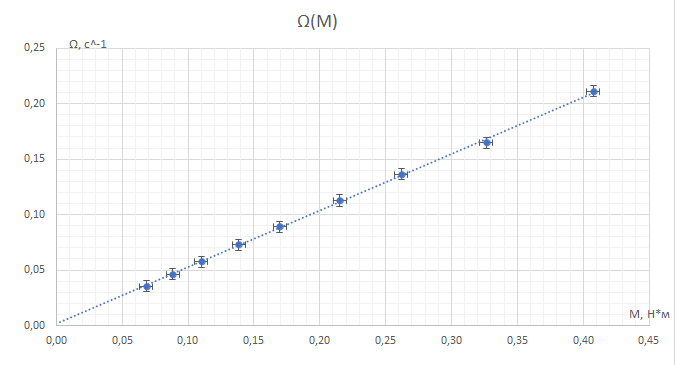
\includegraphics[width=15cm, height=9cm]{1.2.5_gr_1}
\caption{График 1}
\label{gr:1}
\end{figure}
\large$\alpha=\frac{<\Omega{M}>-<\Omega><M>}{<M^2>-<M>^2}=0.512\frac{1}{c*\text{кг}}$ \hfill \break
\large $\sigma_{\alpha}=\sqrt{\frac{1}{7}(\frac{<{\Omega}^2>-<\Omega>^2}{<{\Omega}^2>-<\Omega>^2}-{\alpha}^2)}=0,005\frac{1}{c*\text{кг}}$ \hfill \break
\large $b=<\Omega>-\alpha<M>=0,00128 c^{-1}$ \hfill \break
\large $\sigma_{b}=\sigma_{\alpha}\sqrt{<M^2>}=0,00211c^{-1}$ \hfill \break
5)\par Снимем характеристики цилиндра и посчитаем его момент инерции по формуле (10) \hfill \break
$M_{\text{ц}}$ = 1617.8 г \;\;\;\;\;\; $\Delta{M_{\text{ц}}}$ = 0,3 г \hfill \break
d = 78.4 мм \;\;\;\;\; $\Delta{d}$ = 0.1 мм \hfill \break
где m - масса цилиндра, d - его диаметр \hfill 
\par Тогда момент инерции цилиндра $I_{\text{ц}}=\frac{M_{\text{ц}}R^2}{2}=\frac{M_{\text{ц}}d^2}{8}$ \hfill \break
$I_{0}=I_{\text{ц}}\frac{T^{2}_{0}}{T^{2}_{\text{ц}}}=\frac{M_{\text{ц}}d^2T^{2}_{0}}{8T^{2}_{\text{ц}}}$ \hfill \break
$T_{0} - \text{период колебаний ротора}, T_{\text{ц}} - \text{период колебаний цилиндра}$ \hfill \break
N = 10 \;\;\;\;\; $\Delta{t} = 0.3c$
\begin{center}
\begin{tabular}{|c|c|c|c|}
\hline 
$t_{0}, c$ & $t_{\text{ц}}, с$ & $T_{\text{0}}, с$ & $T_{\text{ц}}, с$ \\ 
\hline 
31.7 & 40.4 & 3.17 & 4.04 \\ 
\hline 
31.8 & 40.2 & 3.18 & 4.02 \\ 
\hline 
31.8 & 40.3 & 3.18 & 4.03 \\ 
\hline 
\end{tabular} 
\end{center}
$<T_{0}> = 3.18c \;\;\;\;\; <T_{\text{ц}}> = 4.03 c$ \hfill \break
$I_{0}=7.7*10^{-4}\text{кг}*\text{м}^2$ \hfill \break
$\sigma_{I_{0}}=I_{0}\sqrt{(\frac{\Delta{M_{\text{ц}}}}{M_{\text{ц}}})^2+4(\frac{\Delta{d}}{d})^2+4(\frac{\Delta{t_{0}}}{t_{0}})^2+4(\frac{\Delta{t_{\text{ц}}}}{t_{\text{ц}}})^2}=0.2*10^{-4}\text{кг}*\text{м}^2$ \hfill \break
$\varepsilon_{I_{0}}=2.6\%$\hfill \break \break
6) \par Ввиду малости b, будем считать подтвержденной теоеретическую зависимость (8). Тогда $\alpha=\frac{gl}{I_{\text{0}}\omega}$ и $\omega=\frac{mgl}{I_{\text{0}}\Omega}=\frac{gl}{I_{\text{0}}\alpha}=\frac{8glT^{2}_{\text{ц}}}{M_{\text{ц}}d^{2}T^{2}_{0}\alpha}$ \hfill \break
$\omega=2524 c^{-1}$ \hfill \break
$\sigma^{\text{приб}}_{\omega}=\omega\sqrt{(\frac{\Delta{m}}{m})^2+(\frac{\Delta{g}}{g})^2+(\frac{\Delta{l}}{l})^2+(\varepsilon_{I_{0}})^2+(\varepsilon_{\Omega})^2}=70 c^{-1}$ \hfill \break
$\sigma^{\text{случ}}_{\omega}=\omega\frac{\sigma_{\alpha}}{\alpha}$ \hfill \break
$\varepsilon_{w}=\frac{\sqrt{(\sigma^{\text{случ}}_{\omega})^2+(\sigma^{\text{приб}}_{\omega})^2}}{\omega}=2.9\%$
$\nu=\frac{\omega}{2\pi}=402 c^{-1}$ \hfill \break
$\varepsilon_{\nu}=\varepsilon_{\omega} = 2.9\%$ \hfill \break
$\sigma_{\nu}=12 c^{-1}$ \hfill \break
7)\par Включим осциллограф и источник, а затем настроим такую частоту, чтобы на экране осциллографа получился эллипс, тем самым определим искомую частоту вращения ротора гироскопа. \hfill \break
$\nu=400\text{Гц}$ \hfill \break
8)\par Определим момент сил трения в оси \hfill \break
\begin{tabular}{|c|c|c|c|c|c|c|c|c|c|c|c|c|c|}
\hline 
$\nu$, Гц & 380 & 370 & 360 & 350 & 340 & 330 & 320 & 310 & 300 & 290 & 280 & 270 \\ 
\hline 
t, c & 20.8 & 46.6 & 72.4 & 99.8 & 127.0 & 154.6 & 183.0 & 212.9 & 244.1 & 274.8 & 305.4 & 338.3 \\ 
\hline 
\end{tabular} 
$\Delta{t}=0.3c$
\begin{figure}[H]
\centering
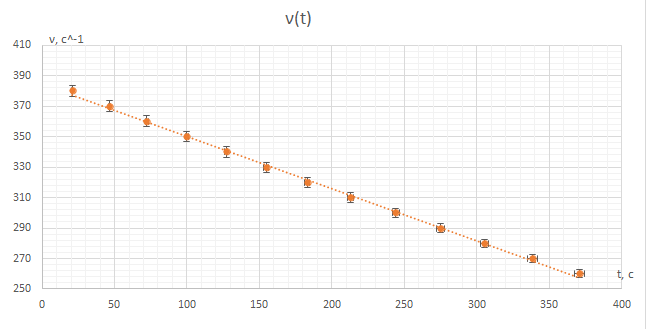
\includegraphics[width=15cm, height=9cm]{1.2.5_gr_2}
\caption{График 1}
\label{gr:2}
\end{figure}
Из (2) и (3)получим следующее соотношение \hfill \break
$\vec{M}=\frac{dI_{0}\vec{\omega}}{dt}$ \hfill \break
Тогда справедливо: \hfill \break
$M_{\text{тр}}=\frac{2\pi{I_{0}}\nu}{t}=2\pi{I_{0}}\beta$ \hfill \break
$\beta$ - коэффициент наклона графика $\nu(t)$ \hfill \break
$\beta=\frac{<\nu{t}>-<\nu><t>}{<t^2>-<t>^2}=-0.343c^{-1}$ \hfill \break
$\sigma_{\beta}=\sqrt{\frac{1}{11}(\frac{<{\nu}^2>-<\nu>^2}{<t^2>-<t>^2}-{\beta}^2)}=0.004c^{-1}$ \hfill \break
$M_{\text{тр}}=1.66*10^{-3}H*\text{м}$ \hfill \break
$\sigma^{\text{приб}}_{M_{\text{тр}}}=M_{\text{тр}}\sqrt{(\frac{\Delta{t}}{<t>})^2+(\frac{d\nu}{<\nu>})^2+(\varepsilon_{I_{0}})^2}=M_{\text{тр}}\varepsilon_{I_{0}}$ \hfill \break
$\sigma^{\text{случ}}_{M_{\text{тр}}}=M_{\text{тр}}\frac{\sigma_{\beta}}{\beta}$ \hfill \break
$\sigma_{M_{\text{тр}}}=0.05*10^{-3}H*\text{м}$ \hfill \break
$\varepsilon_{M_{\text{тр}}}=2,8\%$
\begin{center}
\large Выводы
\end{center}
\par В ходе работы были получены значения фезических величин, описывающих процесс прецессии уравновешенного гироскопа. Значения получены с приемлемой точностью: максимальная относительная погрешность составила $2.9\%$ при определении частоты вращения оси гироскопа. Значительный вклад в нее внесла погрешность измерения времени крутильных колебаний ротора и цилиндра.
\par Наряду с погрешность значительный вклад в погрешность измерения $M_{\text{тр}}$ внесла случайная погрешность. Это может говорить о том, что хотя момент сил трения в оси и угловое ускорение вращения можно считать постоянным при большой частоте вращения, при затухании вращения, уменьшается и значение момента сил трения, из-за чего зависимость при дальнейших измерениях уже нельзя считать линейной.
\par Установлено, что момент сил трения действительно много меньше моментов внешних сил, исследуемых в данной работе. В частности, момент сил трения в среднем на 2 порядка меньше момента силы тяжести подвешенных грузов 
\par В ходе работы были эксперементально подтверждены теоретические зависимости, описывающие процесс прецессии уравновешенного гироскопа.

\end{document}